\subsection*{Poppy Humanoid}
\begin{figure}[ht]
    \centering
    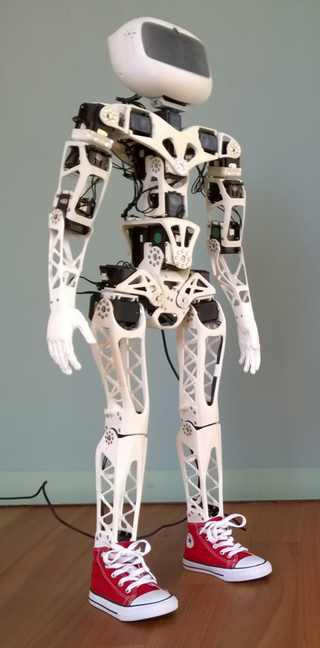
\includegraphics[width=0.35\textwidth]{chapter2/images/PoppyHumanoid1.png}
    \caption{หุ่นยนต์ฮิวมานอยด์ป๊อปปี้}
    \label{fig:poppy_humanoid}
\end{figure}
หุ่นยนต์ฮิวมานอยด์ป๊อปปี้ ถูกสร้างขึ้นมาเพื่อใช้ในงานศิลปะ การวิจัยและการศึกษาโดยเฉพาะ 
หุ่นยนต์ป๊อปปี้ประกอบด้วยส่วนของฮาร์ทแวร์และซอฟแวร์ที่เปิดเป็นโอเพนซอร์ซให้ผู้ที่สนใจสามารถเข้ามาศึกษาได้
โปรแกรมของหุ่นยนต์ใช้โมดูลที่มีชื่อว่า Pypot ที่เป็นส่วนเสริมของภาษา Python ในการพัฒนาซอฟแวร์
ทุกคนสามารถเข้าถึงข้อมูลเชิงเทคนิคของหุ่นยนต์ฮิวมานอยด์ป๊อปปี้ได้ เช่น ส่วนรายละเอียดการทำงาน
คลิปวีดีโอสอนการประกอบ การใช้ระบบจำลอง และการพัฒนาต่างๆผ่านทางเว็บไซต์ http://www.poppy-project.org 
หุ่นยนต์ป๊อปปี้มีส่วนของโครงสร้างที่ผลิตมาจากพลาสติด PLA และ ABS โดยใช้เทคนิคการขึ้นรูปด้วยเครื่องพิมพ์สามมิติ
ตัวขับเคลื่อนข้อต่อต่างๆใช้เป็น Dynamixel Digital Servo และควบคุมคำสั่งของตัวขับเคลื่อนด้วย 
คอมพิวเตอร์ขนาดเล็ก Odroid UX4 ใช้ระบบปฎิบัติการ Ubuntu 14.04 
ตัวของหุ่นยนต์มีความสูง 83 เซนติเมตร น้ำหนัก 3.5 กิโลกรัม 
ใช้เซนเซอร์วัดมุมเอียงเป็น IMU ที่มีองศาอิสระเท่ากับ 9 องศาอิสระ ในการควบคุมเสถียรภาพในการเดินของตัวเอง
มีองศาอิสระหรือจำนวนตัวขับเคลื่อนทั้งหมด 25 องศา ประกอบไปด้วย ขาข้างละ 6 องศาอิสระ แขนข้างละ 4 องศาอิสระ 
ลำตัว 3 องศาอิสระ และ หัว 2 องสาอิสระ\ref{PoppyHumanoid,https://www.poppy-project.org/en/}

\clearpage
\subsection*{iCub Humanoid}
\begin{figure}[ht]
    \centering
    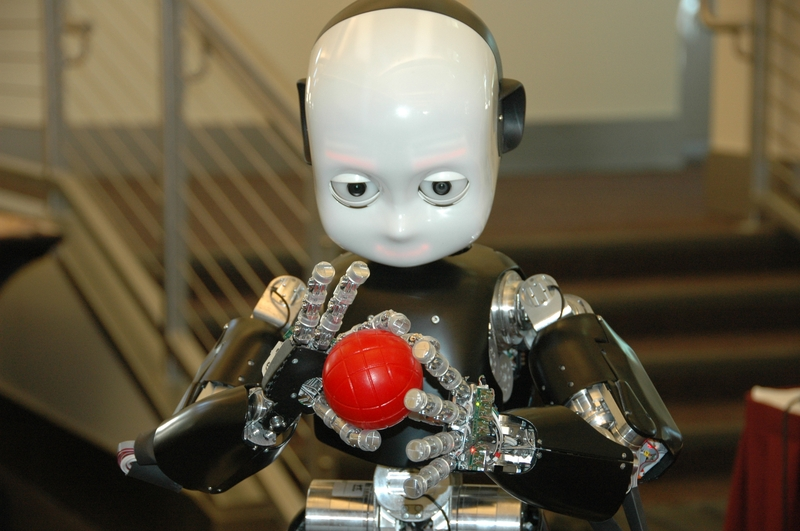
\includegraphics[width=0.6\textwidth]{chapter2/images/icub-1.jpg}
    \caption{หุ่นยนต์ฮิวมานอยด์ไอคัพ}
    \label{fig:icub_humanoid}
\end{figure}
หุ่นยนต์ฮิวมานอยด์ไอคัพ ถูกออกแบบโดยมหาวิทยาลัยหลายแห่งในยุโรปรวมกลุ่มกันขึ้นมาในชื่อ RobotCub
และถูกสร้างขึ้นโดย Istituto Italiano di Tecnologia (IIT) ตัวหุ่นยนต์ไอคัพนั้นมีความสูงอยู่ที่ 1 เมตร
น้ำหนักโดยรวมทั้งหมดประมาณ 22 กิโลกรัม วัสดุที่ใช้ในการสร้างแตกต่างกันไปในแต่ละส่วนของร่างกายโดยจะใช้
aluminum alloy AI6082 สำหรับส่วนที่ต้องรับภาระความเครียดน้อย ใช้ aluminum alloy 7075 (Ergal) สำหรับส่วนที่ต้องรับภาระความเครียดปานกลางถึงสูง
และใช้ Stainless Steel 17-4PH ในส่วนของเพลาข้อต่อต่างๆเพื่อให้มีความแข็งแรงสูง ตัวหุ่นยนต์ถูกออกแบบให้มีลักษณะเหมือนเด็กอายุ 3-4 ขวบ
ควบคุมโดยใช้บอร์ดไมโครคอนโทรเลอร์เป็นรุ่น PC104 Controller ภาษาที่ใช้ในการพัฒนาใช้เป็นภาษา C++ ในการเขียนโปรแกรม
การติดต่อสื่อสารกับตัวขับเคลื่อนหรือมอเตอร์ตามข้อต่อต่างๆ และเซนเซอร์ ผ่านทางโปรโตคอล CAN Bus เพื่อทำให้ใช้สายน้อยลง
ใช้เส้นเอ็นในการส่งถ่ายแรงขับเคลื่อนไปยังส่วนของข้อต่อส่วนมือและไหล่ นิ้วของหุ่นยนต์ถูกร้อยด้วย สายเคเบิลเคลือบ Teflon อยู่ภายใน
และคลายตัวกลับสู่สภาวะสมดุลได้ด้วยแรงของสปริง เซนเซอร์วัดมุมของข้อต่อแต่ละตัวใช้การออกแบบให้มี Hall-effect ติดอยู่
ช่วยในการอ่านค่าของตำแหน่งและความเร็วที่เกิดขึ้นที่ข้อต่อนั้น หุ่นยนต์ไอคัพมีองศาอิสระรวมกันทั้งหมด 53 องศาอิสระ
ประกอบไปด้วย แขนข้างละ 7 องศาอิสระ มือข้างละ 9 องศาอิสระ หัว 6 องศาอิสระ ลำตัว 3 องศาอิสระ และขาข้างละ 6 องศาอิสระ
ในส่วนของหัวจะประกอบไปด้วย กล้องสองตัวเพื่อทำสเตอริโอวิชั่น ไมโครโฟนสำหรับรับเสียงจากสภาพแวดล้อมภายนอก
และไฟแสดงอารมณ์บริเวณปากและคิ้ว หุ่นยนต์นี้ไม่ได้ถูกออกแบบให้มีการทำงานเป็นแบบอัตโนมัติ ซึ่งก็คือตัวหุ่นยนต์นั้นไม่มีแบตเตอรี่ภายในตัว
แต่ใช้แหล่งพลังงานจากภายนอกโดยการส่งเข้าไปผ่านสายเคเบิล และเชื่อมต่อกับอินเทอร์เน็ตผ่านสายแลน (LAN)
\ref{iCubHumanoid,http://www.icub.org/}

\clearpage
\subsection*{Darwin-OP Humanoid}
\begin{figure}[ht]
    \centering
    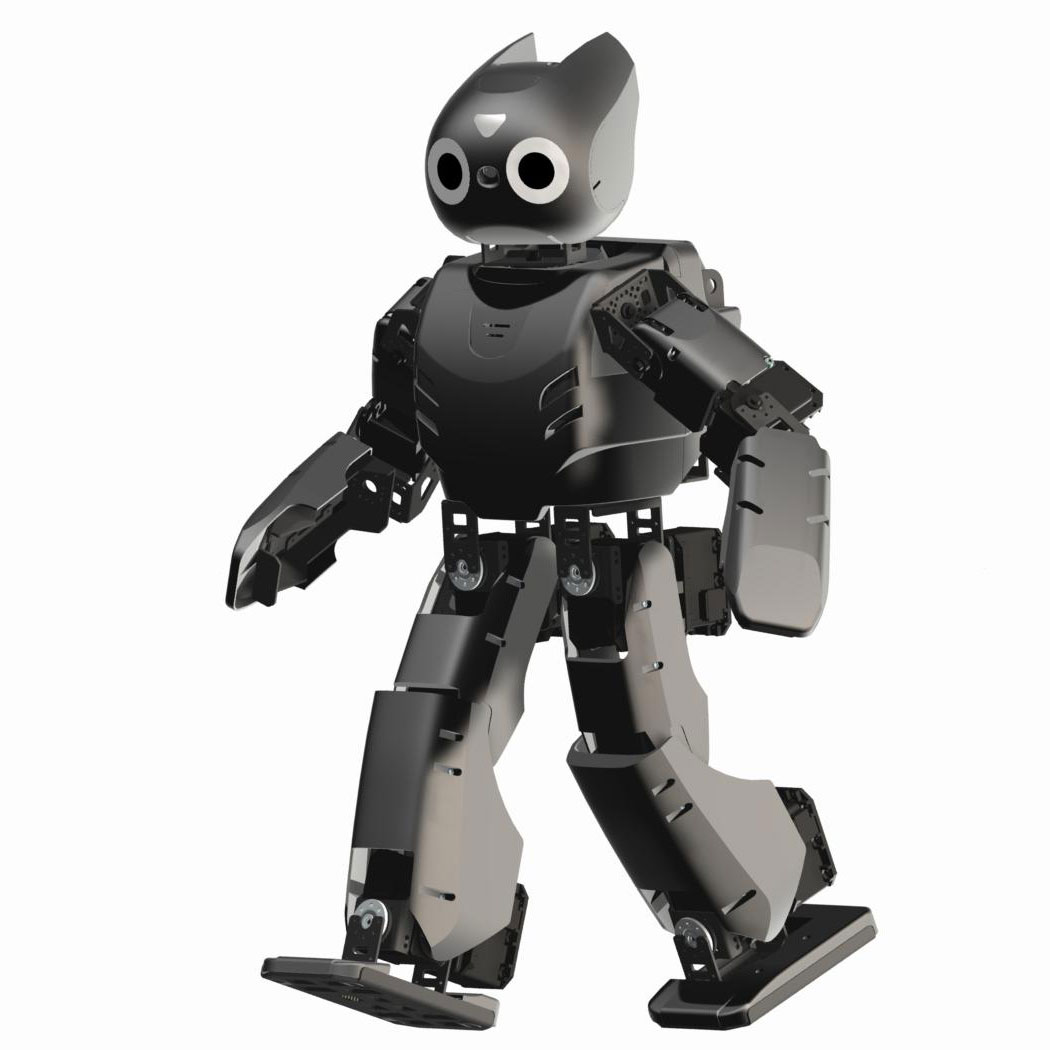
\includegraphics[width=0.55\textwidth]{chapter2/images/Darwin_OP_6.jpg}
    \caption{หุ่นยนต์ฮิวมานอยด์ดาร์วิน}
    \label{fig:darwin_humanoid}
\end{figure}
หุ่นยนต์ฮิวมานอยด์ดาร์วิน (Darwin-OP) เป็นชื่อที่ย่อมาจากคำว่า Dynamic Anthropomorphic Robot
with Intelligence–Open Platform
เป็น OpenSource Platform ที่ถูกออกแบบและพัฒนาโดย Korean robot manufacturer Robotis
โดยมีความร่วมมือกับ Virginia polytechnic institude and state university, Purdue university และ University of Pennsylvania
หุ่นยนต์ฮิวมานอยด์ดาร์วินมีความสามารถในการรับภาระโหลดได้สูง เนื่องจากมีการพัฒนามอเตอร์เป็นของตัวเอง อีกทั้งยังมีความสามารถในการเคลื่อนที่แบบ
พลวัต (Dynamic) หุ่นยนต์ดาร์วิน มีองศาอิสระทั้งหมด 20 องศาอิสระ ซึ่งประกอบไปด้วย ขาข้างละ 6 องศาอิสระ แขนข้างละ 3 องศาอิสระ และหัว 2 องศาอิสระ
ขับเคลื่อนข้อต่อต่างๆด้วยเซอร์โวมอเตอร์ Dynamixel MX-28T ที่มีการเชื่อมต่อแบบ RS485 ในการประหยัดสายที่ใช้ในการสั่งการ มอเตอร์แต่ละตัวมีเซนเซอร์วัดตำแหน่ง 
และความเร็วอยู่ภายใน ตัวหุ่นยนต์มีความสูงทั้งหมด 45 เซนติเมตร มีน้ำหนักโดยประมาณ 2.9 กิโลกรัม
ระบบภายในใช้คอมพิวเตอร์ขนาดเล็กเป็น 1.6 GHz Intel Atom Z530 (32 bit) ใช้คอนโทรเลอร์ ARM CortexM3 STM32F103RE 72 MHz 
และมีเซนเซอร์วัดมุมเอียงเป็น 3-axis gyro, 3-axis accelerometer เพื่อช่วยในการควบคุมเสถียรภาพในการเดิน
\ref{Darwin-OP Humanoid Research Robot,http://www.trossenrobotics.com/p/darwin-OP-Deluxe-humanoid-robot.aspx}

\clearpage
\subsection*{Nao Humanoid}
\begin{figure}[ht]
    \centering
    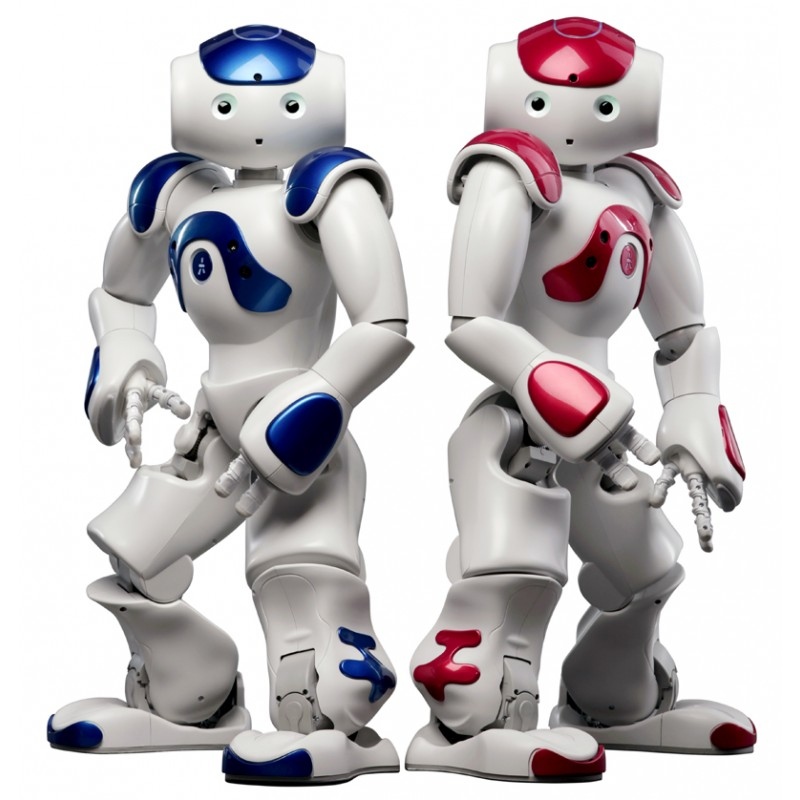
\includegraphics[width=0.55\textwidth]{chapter2/images/nao.jpg}
    \caption{หุ่นยนต์ฮิวมานอยด์นาโอะ}
    \label{fig:nao_humanoid}
\end{figure}
หุ่นยนต์ฮิวมานอยด์นาโอะ เป็นหุ่นยนต์ฮิวมานอยด์ขนาดกลาง ถูกผลิตมาจากประเทศฝรั่งเศษ พัฒนาโดยบริษัท Aldebaran Robotics เมื่อปี 2004 และในปี 2007
หุ่นยนต์ฮิวมานอยด์นาโอะได้นำไปแทนที่หุ่นยนต์สุนัขของ Sony ชื่อ Aibo ขณะถูกใช้ในรายการแข่งขัน RoboCup Standard Platform League (SPL) หุ่นยนต์นาโอะได้ถูกนำไปใช้ใน Robocup 2008 และ 2009 
หุ่นยนต์นาโอะถูกพัฒนาออกมาหลายรุ่นมีองศาอิสระตั้งแต่ 14 องศาอิสระ 21 องศาอิสระ และ 25 องศาอิสระ สำหรับเพื่องานวิจัยนั้นมีถึง 25 องศาอิสระ
โดยเพิ่มเติมมือสองข้างเอาเข้าไปเพื่อให้สามารถหยิบจับสิ่งของได้ ภายในหุ่นยนต์ถูกควบคุมด้วยระบบปฎิบัติการ NAO 2.0 (Linux-based) ตัวหุ่นยนต์มีความสูง 58 เซนติเมตร 
น้ำหนัก 4.3 กิโลกรัม ส่วนเซนเซอร์การรับรู้ต่างๆจะประกอบไปด้วย เซนเซอร์วัดมุมเอียง 3-axis gyro, 3-axis accelerometer, Ultrasound captors, ไมโครโฟน 4 ตัว ลำโพง 2 ตัว กล้อง 2 ตัว เพื่อใช้ประโยชน์ในการทำงานวิจัยต่างๆ
ตอนนี้ความสามารถของหุ่นยนต์นาโอะที่ทำได้คือ สามารถเทน้ำส้มได้ เดินขึ้นลงบันไดและทางลาดชันได้ ระหว่างการเดินนั้นสามารถวางแผนการวางเท้าได้อย่างรวดเร็ว
อีกทั้งยังสามารถที่จะเดินหลบหลีกสิ่งกีดขวางได้ด้วย
\ref{Who is NAO?,https://www.softbankrobotics.com/emea/en/robots/nao}

\clearpage
\subsection*{Wabot}
\begin{figure}[ht]
    \centering
    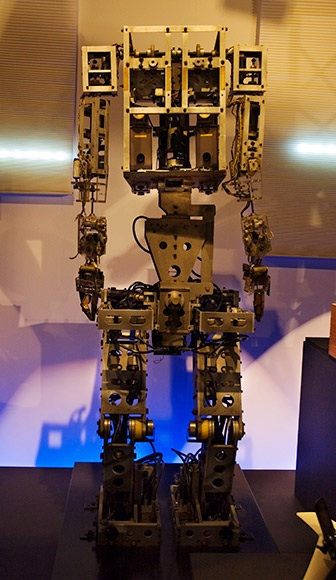
\includegraphics[width=0.45\textwidth]{chapter2/images/wabot.jpg}
    \caption{หุ่นยนต์ฮิวมานอยด์วาบอท}
    \label{fig:wabot_humanoid}
\end{figure}
หุ่นยนต์ฮิวมานอยด์มีการพัฒนาในช่วงแรกเริ่มมาตั้งแต่ปี 1973 หุ่นยนต์ฮิวมานอยด์ ตัวแรกชื่อ Wabot-1 เริ่มสร้างโดยมหาวิทยาลัย Waseda ที่ประเทศญี่ปุ่น ตัวของหุ่นยนต์มีความสูง 180 เซนติเมตร
น้ำหนัก 210 กิโลกรัม โดยหุ่นยนต์สามารถติดต่อสื่อสารกับมนุษย์ได้ด้วยภาษาญี่ปุ่น สามารถวัดระยะและทิศทางได้โดยใช้การรับรู้ผ่านทางตาและหูเทียม หุ่นยนต์ Wabot-1 นั้นสามารถเดินได้ด้วยขาของตนเองที่มีสองข้าง
สามารถหยิบและเคลื่อนย้ายวัตถุด้วยมือ ต่อมาในปี 1984 มหาวิทยาลัย Waseda ได้พัฒนาหุ่นยนต์ฮิวมานอยด์ที่ชื่อ Wabot-2 โดยหุ่นยนต์สามารถสื่อสารกับมนุษย์ได้ สามารถอ่านโน๊ตเพลงและเล่นดนตรีโดยใช้ electronic organ แบบง่ายๆได้
และในปี 1985 บริษัท Hitachi ได้สร้างหุ่นยนต์ WHL-11 ที่มีสองขาเหมือนมนุษย์ ซึ่งสามารถเดินแบบสมดุลสถิต (Static Walking) บนพื้นราบได้ด้วยความเร็ว 13 วินาทีต่อหนึ่งก้าว และสามารถเลี้ยวได้ซ้ายและขวาได้
\ref{Wabot,http://www.humanoid.waseda.ac.jp/booklet/kato_2.html}